% Options for packages loaded elsewhere
\PassOptionsToPackage{unicode}{hyperref}
\PassOptionsToPackage{hyphens}{url}
\PassOptionsToPackage{dvipsnames,svgnames,x11names}{xcolor}
%
\documentclass[
  letterpaper,
  DIV=11,
  numbers=noendperiod]{scrartcl}

\usepackage{amsmath,amssymb}
\usepackage{iftex}
\ifPDFTeX
  \usepackage[T1]{fontenc}
  \usepackage[utf8]{inputenc}
  \usepackage{textcomp} % provide euro and other symbols
\else % if luatex or xetex
  \usepackage{unicode-math}
  \defaultfontfeatures{Scale=MatchLowercase}
  \defaultfontfeatures[\rmfamily]{Ligatures=TeX,Scale=1}
\fi
\usepackage{lmodern}
\ifPDFTeX\else  
    % xetex/luatex font selection
\fi
% Use upquote if available, for straight quotes in verbatim environments
\IfFileExists{upquote.sty}{\usepackage{upquote}}{}
\IfFileExists{microtype.sty}{% use microtype if available
  \usepackage[]{microtype}
  \UseMicrotypeSet[protrusion]{basicmath} % disable protrusion for tt fonts
}{}
\makeatletter
\@ifundefined{KOMAClassName}{% if non-KOMA class
  \IfFileExists{parskip.sty}{%
    \usepackage{parskip}
  }{% else
    \setlength{\parindent}{0pt}
    \setlength{\parskip}{6pt plus 2pt minus 1pt}}
}{% if KOMA class
  \KOMAoptions{parskip=half}}
\makeatother
\usepackage{xcolor}
\setlength{\emergencystretch}{3em} % prevent overfull lines
\setcounter{secnumdepth}{5}
% Make \paragraph and \subparagraph free-standing
\ifx\paragraph\undefined\else
  \let\oldparagraph\paragraph
  \renewcommand{\paragraph}[1]{\oldparagraph{#1}\mbox{}}
\fi
\ifx\subparagraph\undefined\else
  \let\oldsubparagraph\subparagraph
  \renewcommand{\subparagraph}[1]{\oldsubparagraph{#1}\mbox{}}
\fi


\providecommand{\tightlist}{%
  \setlength{\itemsep}{0pt}\setlength{\parskip}{0pt}}\usepackage{longtable,booktabs,array}
\usepackage{calc} % for calculating minipage widths
% Correct order of tables after \paragraph or \subparagraph
\usepackage{etoolbox}
\makeatletter
\patchcmd\longtable{\par}{\if@noskipsec\mbox{}\fi\par}{}{}
\makeatother
% Allow footnotes in longtable head/foot
\IfFileExists{footnotehyper.sty}{\usepackage{footnotehyper}}{\usepackage{footnote}}
\makesavenoteenv{longtable}
\usepackage{graphicx}
\makeatletter
\def\maxwidth{\ifdim\Gin@nat@width>\linewidth\linewidth\else\Gin@nat@width\fi}
\def\maxheight{\ifdim\Gin@nat@height>\textheight\textheight\else\Gin@nat@height\fi}
\makeatother
% Scale images if necessary, so that they will not overflow the page
% margins by default, and it is still possible to overwrite the defaults
% using explicit options in \includegraphics[width, height, ...]{}
\setkeys{Gin}{width=\maxwidth,height=\maxheight,keepaspectratio}
% Set default figure placement to htbp
\makeatletter
\def\fps@figure{htbp}
\makeatother

\KOMAoption{captions}{tableheading}
\makeatletter
\makeatother
\makeatletter
\makeatother
\makeatletter
\@ifpackageloaded{caption}{}{\usepackage{caption}}
\AtBeginDocument{%
\ifdefined\contentsname
  \renewcommand*\contentsname{Table of contents}
\else
  \newcommand\contentsname{Table of contents}
\fi
\ifdefined\listfigurename
  \renewcommand*\listfigurename{List of Figures}
\else
  \newcommand\listfigurename{List of Figures}
\fi
\ifdefined\listtablename
  \renewcommand*\listtablename{List of Tables}
\else
  \newcommand\listtablename{List of Tables}
\fi
\ifdefined\figurename
  \renewcommand*\figurename{Figure}
\else
  \newcommand\figurename{Figure}
\fi
\ifdefined\tablename
  \renewcommand*\tablename{Table}
\else
  \newcommand\tablename{Table}
\fi
}
\@ifpackageloaded{float}{}{\usepackage{float}}
\floatstyle{ruled}
\@ifundefined{c@chapter}{\newfloat{codelisting}{h}{lop}}{\newfloat{codelisting}{h}{lop}[chapter]}
\floatname{codelisting}{Listing}
\newcommand*\listoflistings{\listof{codelisting}{List of Listings}}
\makeatother
\makeatletter
\@ifpackageloaded{caption}{}{\usepackage{caption}}
\@ifpackageloaded{subcaption}{}{\usepackage{subcaption}}
\makeatother
\makeatletter
\@ifpackageloaded{tcolorbox}{}{\usepackage[skins,breakable]{tcolorbox}}
\makeatother
\makeatletter
\@ifundefined{shadecolor}{\definecolor{shadecolor}{rgb}{.97, .97, .97}}
\makeatother
\makeatletter
\makeatother
\makeatletter
\makeatother
\ifLuaTeX
  \usepackage{selnolig}  % disable illegal ligatures
\fi
\IfFileExists{bookmark.sty}{\usepackage{bookmark}}{\usepackage{hyperref}}
\IfFileExists{xurl.sty}{\usepackage{xurl}}{} % add URL line breaks if available
\urlstyle{same} % disable monospaced font for URLs
\hypersetup{
  pdftitle={MKTG100 Numeracy},
  pdfauthor={AD},
  colorlinks=true,
  linkcolor={blue},
  filecolor={Maroon},
  citecolor={Blue},
  urlcolor={Blue},
  pdfcreator={LaTeX via pandoc}}

\title{MKTG100 Numeracy}
\usepackage{etoolbox}
\makeatletter
\providecommand{\subtitle}[1]{% add subtitle to \maketitle
  \apptocmd{\@title}{\par {\large #1 \par}}{}{}
}
\makeatother
\subtitle{Solutions To Week 8a's Exercises}
\author{AD}
\date{}

\begin{document}
\maketitle
\ifdefined\Shaded\renewenvironment{Shaded}{\begin{tcolorbox}[sharp corners, borderline west={3pt}{0pt}{shadecolor}, frame hidden, boxrule=0pt, breakable, interior hidden, enhanced]}{\end{tcolorbox}}\fi

\renewcommand*\contentsname{Table of contents}
{
\hypersetup{linkcolor=}
\setcounter{tocdepth}{3}
\tableofcontents
}
\hypertarget{week-8a}{%
\section*{Week 8a}\label{week-8a}}
\addcontentsline{toc}{section}{Week 8a}

\hypertarget{fixed-cost-and-variable-cost}{%
\subsection*{1.2. Fixed cost and variable
cost}\label{fixed-cost-and-variable-cost}}
\addcontentsline{toc}{subsection}{1.2. Fixed cost and variable cost}

\textbf{Problem}

The cost of making a one unit of a product is £40. What is the cost to
make 20 units?

Answer:

£40 times 20 = £800

\textbf{Exercise}

Look at the table below.

\begin{figure}

{\centering 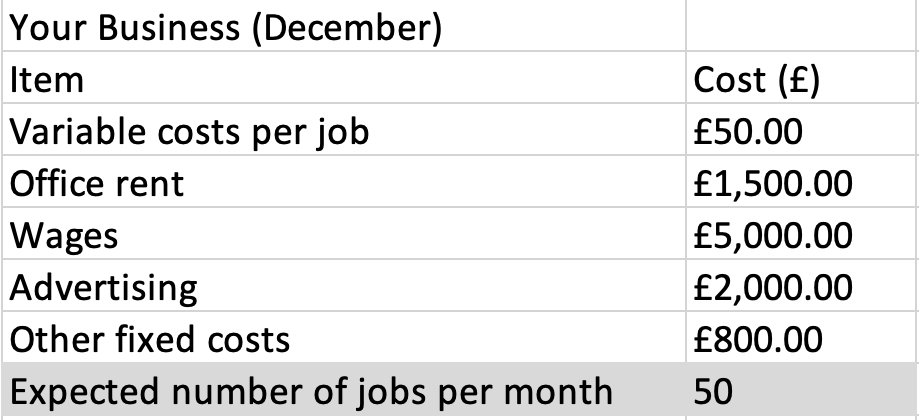
\includegraphics[width=0.6\textwidth,height=\textheight]{images/businesscosts.png}

}

\end{figure}

Calculate total cost.

Answer:

\begin{figure}

{\centering 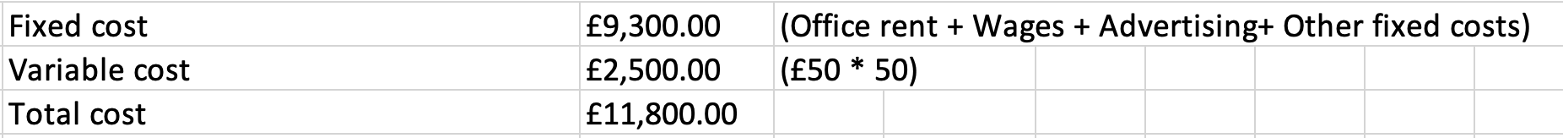
\includegraphics[width=1\textwidth,height=\textheight]{images/totalcost.png}

}

\caption{Total cost}

\end{figure}

\hypertarget{break-even-analysis}{%
\subsection*{Break-even analysis}\label{break-even-analysis}}
\addcontentsline{toc}{subsection}{Break-even analysis}

\textbf{Problem}

You sell a product with a price of £20 per unit. The variable cost of
the product is £10 per unit. The fixed costs associated with the product
is £20,000. How many products should you sell to achieve break-even?

\emph{Answer:}

Fixed cost = £20000

Selling price = £20

Variable cost per product = £10

\begin{align}
Contribution &= Selling \; Price - Variable \; Cost \\
&= £20 - £10 \\
&= £10
\end{align}

Therefore,

\begin{align}
BE \; quantity &= \frac{Fixed \ cost}{Contribution} \\
&= \frac{£20000}{£10} \\
&= 2000
\end{align}

Thus, you should sell 2000 units.

\textbf{Exercises}

\begin{enumerate}
\def\labelenumi{\arabic{enumi}.}
\tightlist
\item
  A company's variable costs per product are £5. The daily fixed costs
  are £100. If the product is sold at £10, calculate the break-even
  quantity.
\end{enumerate}

\emph{Answer}

\begin{align}
Contribution &= Selling \; Price - Variable \; Cost \\
&= £10 - £5 \\
&= £5
\end{align}

Therefore,

\begin{align}
BE \; quantity &= \frac{Fixed \ cost}{Contribution} \\
&= \frac{£100}{£5} \\
&= 20
\end{align}

\begin{enumerate}
\def\labelenumi{\arabic{enumi}.}
\setcounter{enumi}{1}
\tightlist
\item
  If you increase the selling price by 5\%, calculate the new break-even
  quantity.
\end{enumerate}

\emph{Answer}

New selling price = \(105 \% \times £10 = 10.5\)

\begin{align}
Contribution &= Selling \; Price - Variable \; Cost \\
&= £10.5 - £5 \\
& = £5.5
\end{align}

Therefore,

\begin{align}
BE \; quantity &= \frac{Fixed \ cost}{Contribution} \\
&= \frac{£100}{£5.5} \\
&= 18.18 
\end{align}

The BE quantity is 18.18. You can not sell partial units. You may round
up to the next whole number (if you round down, you will incur a profit
loss). Thus, you must sell at least 19 units.



\end{document}
